\documentclass[12pt, letterpaper]{article}
\usepackage[left=2.5cm,right=2.5cm, top=2.5cm, bottom=2.5cm]{geometry}
\usepackage{fancyhdr}
\pagestyle{fancy}
\fancyhead[R]{Flaherty, \thepage}
\renewcommand{\headrulewidth}{2pt}
\setlength{\headheight}{15pt}
\usepackage{lipsum}
\usepackage{amsmath}
\usepackage[makeroom]{cancel}
\usepackage{cancel}
\usepackage{array,polynom}
\newcolumntype{C}{>{{}}c<{{}}} 
\newcolumntype{R}{>{\displaystyle}r}  
\usepackage{xcolor}
\newcommand\Ccancel[2][black]{\renewcommand\CancelColor{\color{#1}}\cancel{#2}}
\usepackage{amssymb}
\usepackage{bbm}
\usepackage{mathrsfs}
\usepackage[toc]{glossaries}
\usepackage{amsthm}
\usepackage{indentfirst}
\usepackage[utf8]{inputenc}
\usepackage[thinc]{esdiff}
\usepackage{graphicx}
\graphicspath{{./images/}}
\usepackage{subfig}
\usepackage{chngcntr}
\usepackage{placeins}
\usepackage{caption}
\usepackage{float}
\usepackage{comment}
\usepackage{sectsty}
\sectionfont{\fontsize{15}{15}\selectfont}
\usepackage{subcaption}
\setlength\abovedisplayskip{0pt}
\usepackage[hidelinks]{hyperref}
\usepackage[nottoc,numbib]{tocbibind}
\renewcommand{\qedsymbol}{\rule{0.7em}{0.7em}}
\newcommand{\Mod}[1]{\ (\mathrm{mod}\ #1)}
\counterwithin{figure}{section}
\usepackage{centernot}
\usepackage{enumitem}  



%Numbering and Math Types%             
\theoremstyle{definition}
\newtheorem{exmp}{Example}
\newtheorem{nonexmp}{Non-Example}
\newtheorem{theorem}{Theorem}[section]
\newtheorem{corollary}{Corollary}[theorem]
\newtheorem{definition}{Definition}[section]
\newtheorem{prop}{Proposition}[section]
\newtheorem{lemma}{Lemma}[theorem]
\numberwithin{equation}{section}
\newenvironment{ex}{
	\par\smallskip 
	\noindent\textit{Example:\hspace{-0.25em}}
	\leftskip=0.5em
}{
	\par\smallskip
	\leftskip=0em
}

\newenvironment{nonex}{
	\par\smallskip
	\noindent\textit{Non-example:\hspace{-0.25em}}
	\leftskip=0.5em 
}{
	\par\smallskip 
	\leftskip=0em 
}

\newcommand{\problem}[1]{\noindent \textbf{Problem \thesection.#1)}}



%References%
\newcommand{\mydef}[1]{(Definition \ref{#1}, Page \pageref{#1})}
\newcommand{\mytheorem}[1]{(Theorem \ref{#1}, Page \pageref{#1})}
\newcommand{\mycor}[1]{(Corollary \ref{#1}, Page \pageref{#1})}
\newcommand{\mylemma}[1]{(Lemma \ref{#1}, Page \pageref{#1})}
\newcommand{\myprob}[1]{(Problem \ref{#1}, Page \pageref{#1})}
\newcommand{\clickableword}[2]{\hyperref[#1]{#2}}



%Commutative Diagrams%
\usepackage{tikz}                     
\usetikzlibrary{arrows}               
\usetikzlibrary{shapes.geometric}  
\usetikzlibrary{calc}
\pgfkeys{/tikz/.cd,
	num vertex/.initial=4,
	num vertex/.get=\vertices,
	num vertex/.store in=\vertices,
	circle radius/.initial=3,
	circle radius/.get=\circleradius,
	circle radius/.store in=\circleradius,
	shift angle/.initial=0,
	shift angle/.get=\shiftangle,
	shift angle/.store in=\shiftangle, 
	at pos/.initial={(0,0)},
	at pos/.get=\position,
	at pos/.store in=\position,
	vertex radius/.initial=1.5pt,
	vertex radius/.get=\vertexradius,
	vertex radius/.store in=\vertexradius,
}
\makeatletter
\def\drawvertices{\tikz@path@overlay{node}}
\makeatother   
\pgfkeys{/tikz/circumference with labels/.code={
		\pgfmathsetmacro\halfcircleradius{\circleradius/2}
		\draw \position circle (\halfcircleradius cm) node[regular polygon, regular polygon sides=\vertices, minimum size=\circleradius cm, draw=none, name={vertex set}] {};
		\foreach \textlabel/\circlecolor [count=\x] in {#1}{
			\node[draw,circle, inner sep=\vertexradius,black, fill=\circlecolor] at (vertex set.corner \x) {};
			\pgfmathparse{\shiftangle-360*(\x-1)/ \vertices}
			\node at ($(vertex set)+(\pgfmathresult:\halfcircleradius)$)[label={[font=\small]\pgfmathresult:$\textlabel$}]{};
		}
	}
}



%Custom command for matrices%
\newcommand{\mymatrix}[1]{
	\renewcommand{\arraystretch}{0.5} 
	\setlength\arraycolsep{3pt}       
	\scalebox{0.90}{                  
		$\begin{bmatrix}
			#1
		\end{bmatrix}$
	}                   
	\renewcommand{\arraystretch}{1.0} 
	\setlength\arraycolsep{6pt}       
}



%underscript for operations%
\newcommand{\+}[1]{+_{\scalebox{.375}{#1}}}
\newcommand{\mult}[1]{\cdot_{\scalebox{.375}{#1}}}



%limits for summands and such%
\newcommand{\mysum}[2]{\sum\limits_{#1}^{#2}}
\newcommand{\mylim}[2]{\lim\limits_{#1}^{#2}}
\newcommand{\myint}[2]{\int\limits_{#1}^{#2}}
\newcommand{\myprod}[2]{\prod\limits_{#1}^{#2}}


%shortcuts for stats and derivatives%
\newcommand{\drv}[2]{\frac{d #1}{d #2}}
\newcommand{\pdrv}[2]{\frac{\partial #1}{\partial #2}}
\newcommand{\samp}[1]{\underset{\sim}{\hat{#1}}}
\newcommand{\estimator}[1]{\underset{\sim}{#1}}
\newcommand{\mom}[1]{\underset{\sim}{#1_{\scalebox{0.35}{MOM}}}}
\newcommand{\mle}[1]{\underset{\sim}{#1_{\scalebox{0.35}{MLE}}}}



%blackboard for letters%
\newcommand{\E}{\mathbb{E}}
\newcommand{\V}{\mathbb{V}}
\newcommand{\R}{\mathbb{R}}
\newcommand{\N}{\mathbb{N}}
\newcommand{\C}{\mathbb{C}}
\newcommand{\Z}{\mathbb{Z}}
\newcommand{\F}{\mathbb{F}}
\newcommand{\Q}{\mathbb{Q}}
\newcommand{\K}{\mathbb{K}}
\newcommand{\1}{\mathbbm{1}}
\newcommand{\Prob}{\mathbbm{P}}

\title{Linear Models HW \# 2}
\author{Liam Flaherty}
\date{\parbox{\linewidth}{\centering%
		Professor Maity\endgraf\bigskip
		NCSU: ST503-651\endgraf\bigskip
		May 27, 2024 \endgraf}}

\begin{document}
\maketitle
\thispagestyle{empty}

	
\newpage\clearpage\noindent


\noindent\textbf{1) \boldmath{Consider the linear model with response vector $y=\mymatrix{y_{1_1}&y_{1_2}&y_{1_3}&y_{2_1}&y_{2_2}&y_{2_3}}^T$, parameter vector is $\beta=\mymatrix{\mu, \alpha_1, \alpha_2, \beta_1, \beta_2, \beta_3}^T$, and model matrix $X$ as follows: $\mymatrix{
	1&1&0&1&0&0\\
	1&1&0&0&1&0\\
	1&1&0&0&0&1\\
	1&0&1&1&0&0\\
	1&0&1&0&1&0\\
	1&0&1&0&0&1}$.}}

\vspace{\baselineskip}
\noindent\textbf{\boldmath{a. What is the rank of $X$?}}
\vspace{\baselineskip}

Four. This can be seen by inspection, since the first column is the sum of the last three columns (which are all clearly independent), and since only one of the second or third columns can also be independent (the last three columns less the second column yields the third column).



\vspace{\baselineskip}
\noindent\textbf{\boldmath{b. Write the normal equations. Explain why the normal equations have infinitely many solutions.}}
\vspace{\baselineskip}

In general, the normal equation is $(X^TX)\beta=X^T y$. Since $X$ has less than full column rank (by part a), $X^TX$ is not invertible. We must then use a generalized inverse $(X^TX)^-$ to arrive at our estimate, $\samp{\beta}=(X^TX)^-X^T y$. And while $(X^TX)^-$ is not unique, $\samp{\beta}$ is.


\vspace{\baselineskip}
\noindent\textbf{\boldmath{c. Show that $\alpha_1-\alpha_2$ is estimable. Don't use any software.}}
\vspace{\baselineskip}

A linear function $C^T \beta$ is estimable if and only if $C$ is in the column space of $X^T$ ($C^T$ is in the row space of $X$). Here, our function is $C^T\beta=\alpha_1-\alpha_2=\mymatrix{0&1&-1&0&0&0}\beta$, so $C^T=\mymatrix{0&1&-1&0&0&0}$. This is in the row space of $X$, since it is the first row of $X$ less the fourth row of $X$; $\mymatrix{0&1&-1&0&0&0}=\mymatrix{1&1&0&1&0&0}-\mymatrix{1&0&1&0&1&0}\implies C^T=X_{\cdot,1}-X_{\cdot,4}$.




\vspace{\baselineskip}
\noindent\textbf{\boldmath{d. Show that $\beta_1-2\beta_2+\beta_3$ is estimable. Don't use any software.}}
\vspace{\baselineskip}

In the same vein as part c, our function is $C^T \beta=\beta_1-2\beta_2+\beta_3=\mymatrix{0&0&0&1&-2&1}\beta$. This is in the row space of $X$, since it is the first row of $X$, less two of the second row of $X$, plus the third row of $X$; $\mymatrix{0&0&0&1&-2&1}=\mymatrix{1&1&0&1&0&0}-2\mymatrix{1&1&0&0&1&0}+\mymatrix{1&1&0&0&0&1}$.


\vspace{\baselineskip}
\noindent\textbf{\boldmath{e. Use R to check your answers in part c and d above.}}
\vspace{-0.25cm}

\begin{figure}[H]
	\centering
	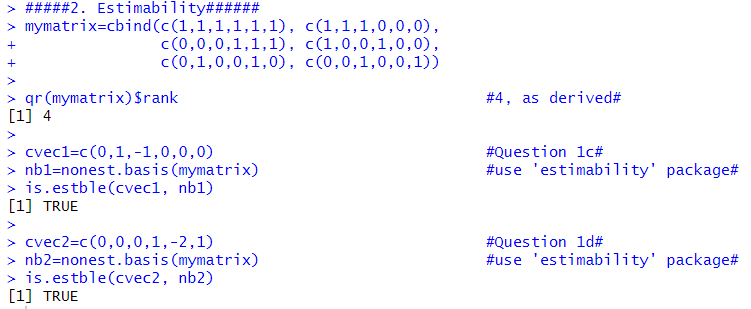
\includegraphics[width=12cm]{Estimability R Code}
\end{figure}



\newpage
\noindent\textbf{\boldmath{
2) The dataset `teengam' concerns a study of teenage gambling in Britian. Fit a regression model with the expenditure on gambling as the response and the sex, status, income, and verbal score as predictors.}}

\vspace{\baselineskip}
\noindent\textbf{\boldmath{a. Present the output. What percentage of variation in the response is explained by these predictors?}}
\vspace{\baselineskip}

The predictors explain about 52.7\% of the variation in the response.

\begin{figure}[H]
	\centering
	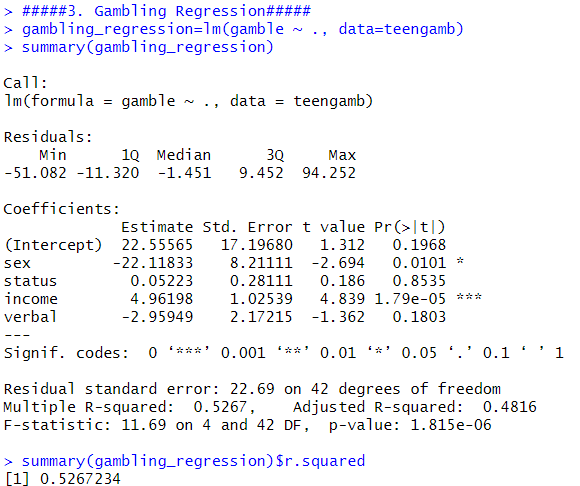
\includegraphics[width=12cm]{Gambling R Square}
\end{figure}


\vspace{\baselineskip}
\noindent\textbf{\boldmath{b. Which observation has the largest (positive) residual? Give the case number.}}
\vspace{-0.25cm}

The twenty-fourth person in the database had the largest positive residual. The model underestimated his predicted annual spending on gambling by over 94 pounds.

\begin{figure}[H]
	\centering
	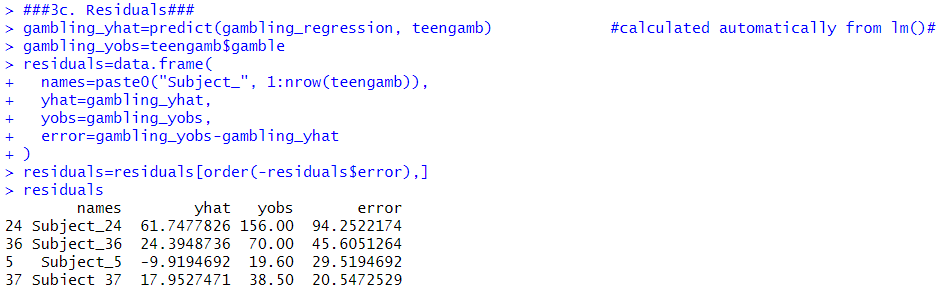
\includegraphics[width=14cm]{Gambling Residual}
\end{figure}


\vspace{\baselineskip}
\noindent\textbf{\boldmath{c. Compute the mean and median of the residuals.}}
\vspace{\baselineskip}

The mean residual was virtually zero. The median residual was about -1.45.

\begin{figure}[H]
	\centering
	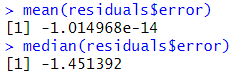
\includegraphics[width=4cm]{Gambling Mean Residual}
\end{figure}

\vspace{\baselineskip}
\noindent\textbf{\boldmath{d. Compute the correlation of the residuals with the fitted values.}}
\vspace{\baselineskip}

The residuals and fitted values were largely uncorrelated.

\begin{figure}[H]
	\centering
	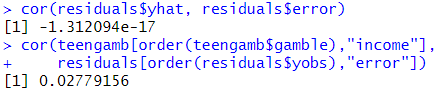
\includegraphics[width=6cm]{Gambling Correlation}
\end{figure}



\vspace{\baselineskip}
\noindent\textbf{\boldmath{e. Compute the correlation of the residuals with the income.}}
\vspace{\baselineskip}

The correlation of the residuals with income was about 0.03.

\begin{figure}[H]
	\centering
	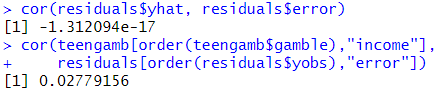
\includegraphics[width=6cm]{Gambling Correlation}
\end{figure}


\vspace{\baselineskip}
\noindent\textbf{\boldmath{f. For all other predictors held constant, what would be the difference in predicted expenditure on gambling for a male compared to a female?}}
\vspace{\baselineskip}

Since male/female is binary (female is coded as `1'), if all other predictors are held constant, then the difference in prediction would be the estimate for the sex variable. In this case, the predictor was about -22.12, so a male would be predicted to spend about 22.12 pounds more annually compared to females.

\begin{figure}[H]
	\centering
	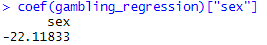
\includegraphics[width=6cm]{Gambling Coef Sex}
\end{figure}


\newpage
\noindent\textbf{\boldmath{3) The dataset `uswages' is drawn as a sample from the Current Population Survey in 1988. Fit a model with weekly wages as the resopnse and years of education and experience as predictors. Report and give a simple interpretation to the regression coefficient for years of education. Now fit the same model but with logged weekly wages. Give an interpretation to the regression coefficient for years of education. Which interpretation is more natural?}}
\vspace{\baselineskip}

The model for the predicted weekly wages is approximately \$50 for every year of education plus \$10 for every year of experience, less about \$240. More specifically, the linear model predicts that with every additional year of education, one would be expected to earn an additional \$51.18 a week (in 1992 dollars, deflated by PCE inflation).


\begin{figure}[H]
	\centering
	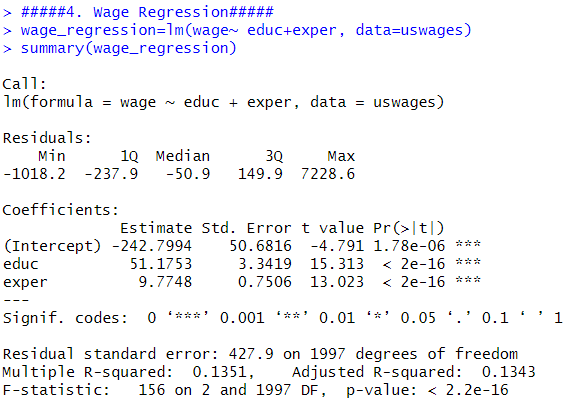
\includegraphics[width=10cm]{Wage Regression}
\end{figure}

In contrast, the same model but with logged weekly wages predicts every additional year of education would be expected to net a person about \$0.09 log-dollars a week. While there is some argument to be made that the positive intercept in the log model makes an interpretation at the extremes more reasonable, in total, the interpretation makes more since when the prediction isn't logged.

\begin{figure}[H]
	\centering
	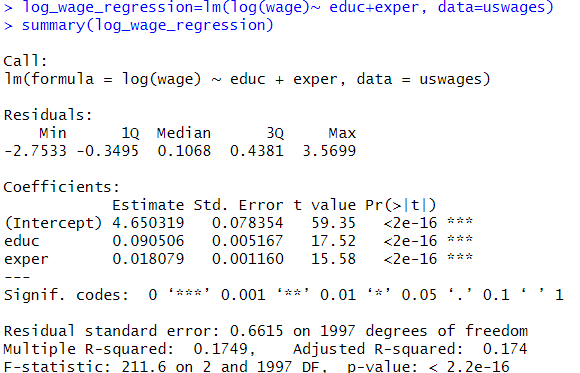
\includegraphics[width=10cm]{Log Wage Regression}
\end{figure}




\newpage
\section*{R Code}

\begin{figure}[H]
	\centering
	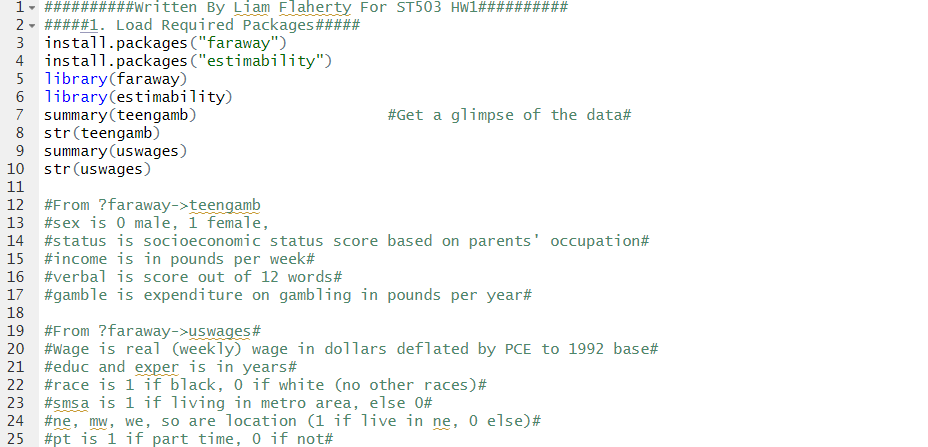
\includegraphics[width=14cm]{Gambling R Code 1}
\end{figure}
\begin{figure}[H]
	\centering
	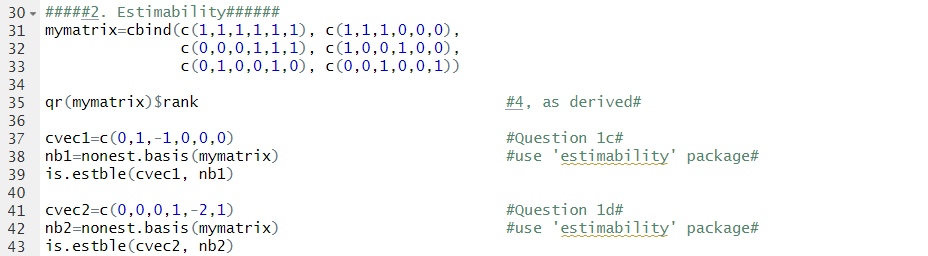
\includegraphics[width=14cm]{Gambling R Code 2}
\end{figure}
\begin{figure}[H]
	\centering
	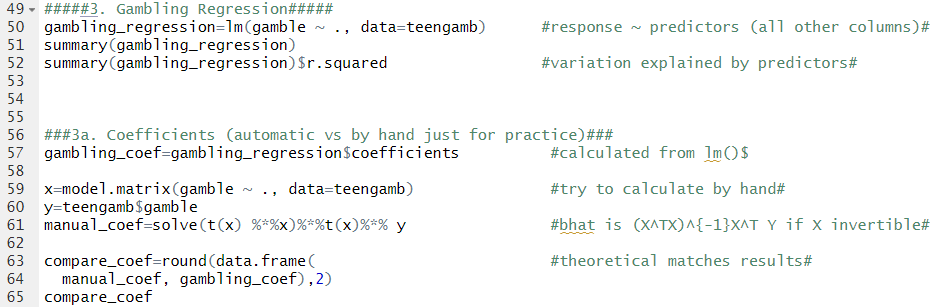
\includegraphics[width=14cm]{Gambling R Code 3}
\end{figure}
\begin{figure}[H]
	\centering
	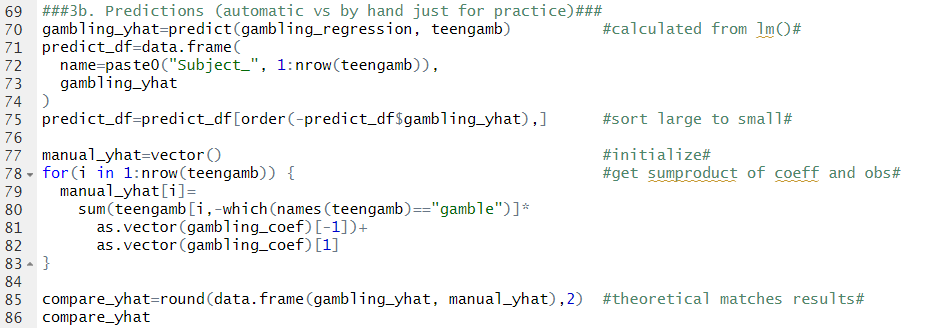
\includegraphics[width=14cm]{Gambling R Code 4}
\end{figure}
\begin{figure}[H]
	\centering
	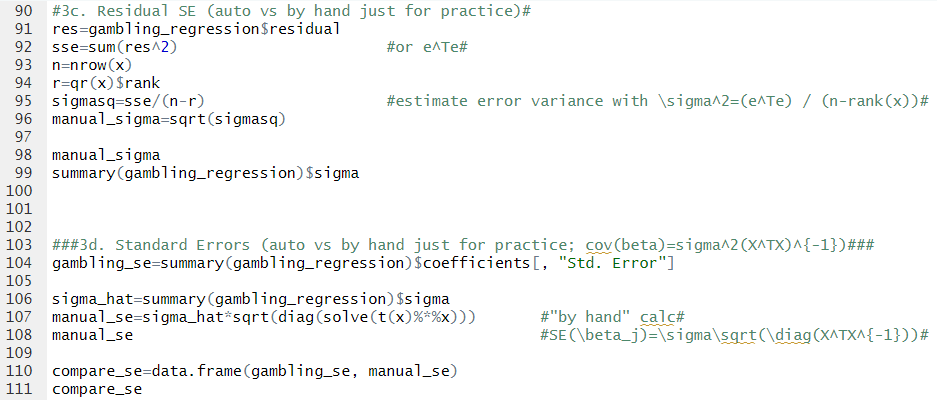
\includegraphics[width=14cm]{Gambling R Code 5}
\end{figure}
\begin{figure}[H]
	\centering
	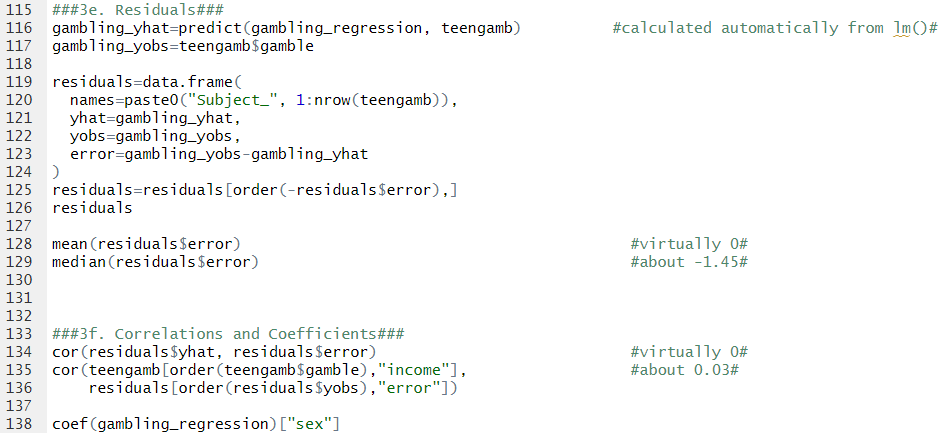
\includegraphics[width=14cm]{Gambling R Code 6}
\end{figure}
\begin{figure}[H]
	\centering
	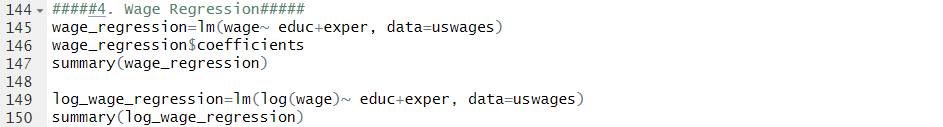
\includegraphics[width=14cm]{Gambling R Code 7}
\end{figure}


\end{document}